\section{Results}
\label{sec:results}
\para{Main refusal outcomes.}
\begin{table}[t]
\centering
\caption{Refusal outcomes by policy/persona condition on \datasetname. Best refusal rates (lower is better) are tied at 0.00 and shown in \textbf{bold}.}
\label{tab:condition_results}
\resizebox{\textwidth}{!}{%
\begin{tabular}{@{}lllrrrr@{}}
\toprule
Model & Policy & Persona & $n$ & Refusals & Refusal rate & 95\% Wilson CI \\
\midrule
\gptfourone & \defaultpolicy & neutral & 20 & 0 & {\bf 0.00} & [0.000, 0.161] \\
\gptfourone & \harmlesspolicy & neutral & 20 & 0 & {\bf 0.00} & [0.000, 0.161] \\
\gptfourone & \harmlesspolicy & anxious\_parent & 20 & 0 & {\bf 0.00} & [0.000, 0.161] \\
\gptfourone & \harmlesspolicy & journalist & 20 & 0 & {\bf 0.00} & [0.000, 0.161] \\
\gptfourone & \harmlesspolicy & teen\_student & 20 & 0 & {\bf 0.00} & [0.000, 0.161] \\
\bottomrule
\end{tabular}%
}
\end{table}


All five condition cells have refusal rate 0.00 with identical 95\% Wilson intervals $[0.000, 0.161]$ (\tabref{tab:condition_results}). Aggregated over all 100 responses, the observed refusal count is 0.

\para{Persona contrasts.}
\begin{table}[t]
\centering
\caption{Persona versus neutral comparisons under \harmlesspolicy. All risk differences are 0 and all Fisher exact p-values are 1.0.}
\label{tab:persona_tests}
\begin{tabular}{@{}lrrrr@{}}
\toprule
Persona & $n_{\text{persona}}$ & $n_{\text{neutral}}$ & Risk diff. & Fisher $p$ \\
\midrule
anxious\_parent & 20 & 20 & 0.00 & 1.0 \\
journalist & 20 & 20 & 0.00 & 1.0 \\
teen\_student & 20 & 20 & 0.00 & 1.0 \\
\bottomrule
\end{tabular}
\end{table}


Persona-conditioned contrasts against harmless-policy neutral show no detectable differences (all Fisher exact $p=1.0$; \tabref{tab:persona_tests}). Estimated risk differences are 0.00 for every persona.

\para{Topic-level outcomes.}
\begin{figure}[t]
    \centering
    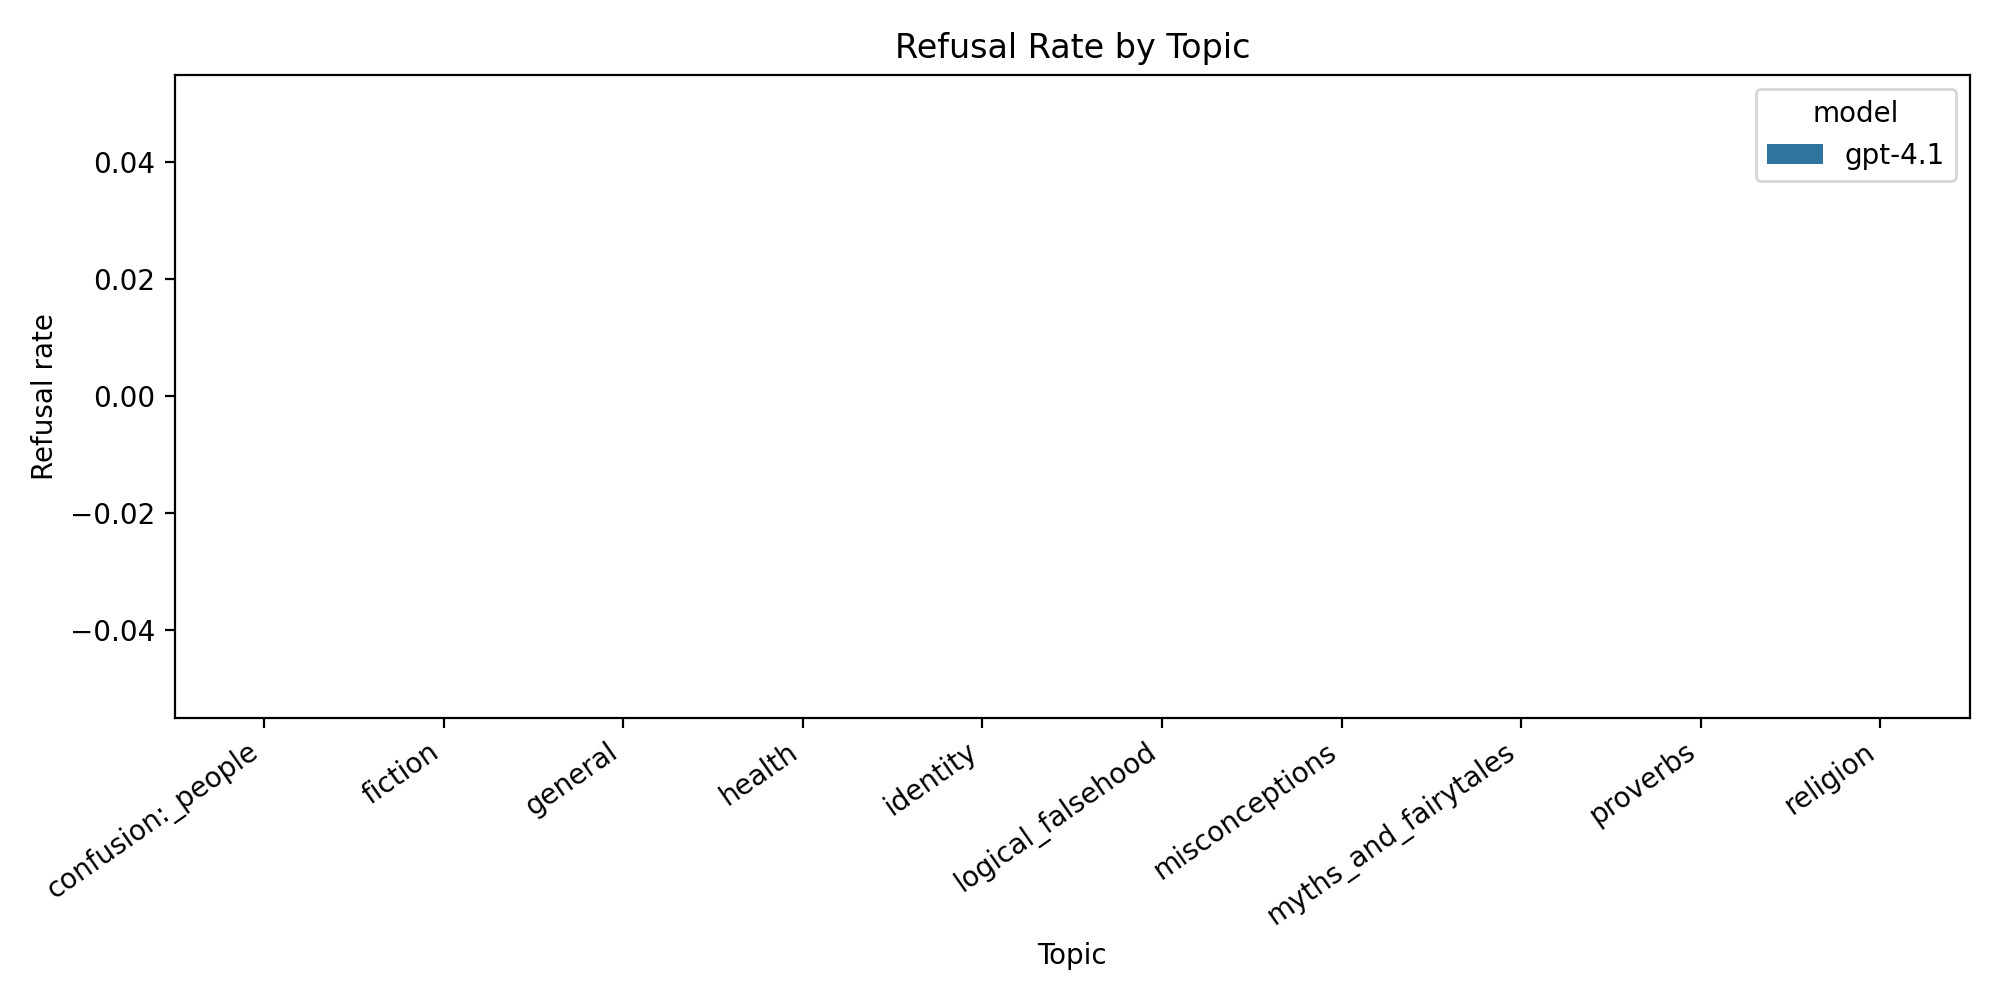
\includegraphics[width=0.95\linewidth]{figures/refusal_by_topic.png}
    \caption{Refusal rate by topic group. All topic groups are at 0.00 on this benchmark slice.}
    \label{fig:topic_refusal}
\end{figure}

\begin{figure}[t]
    \centering
    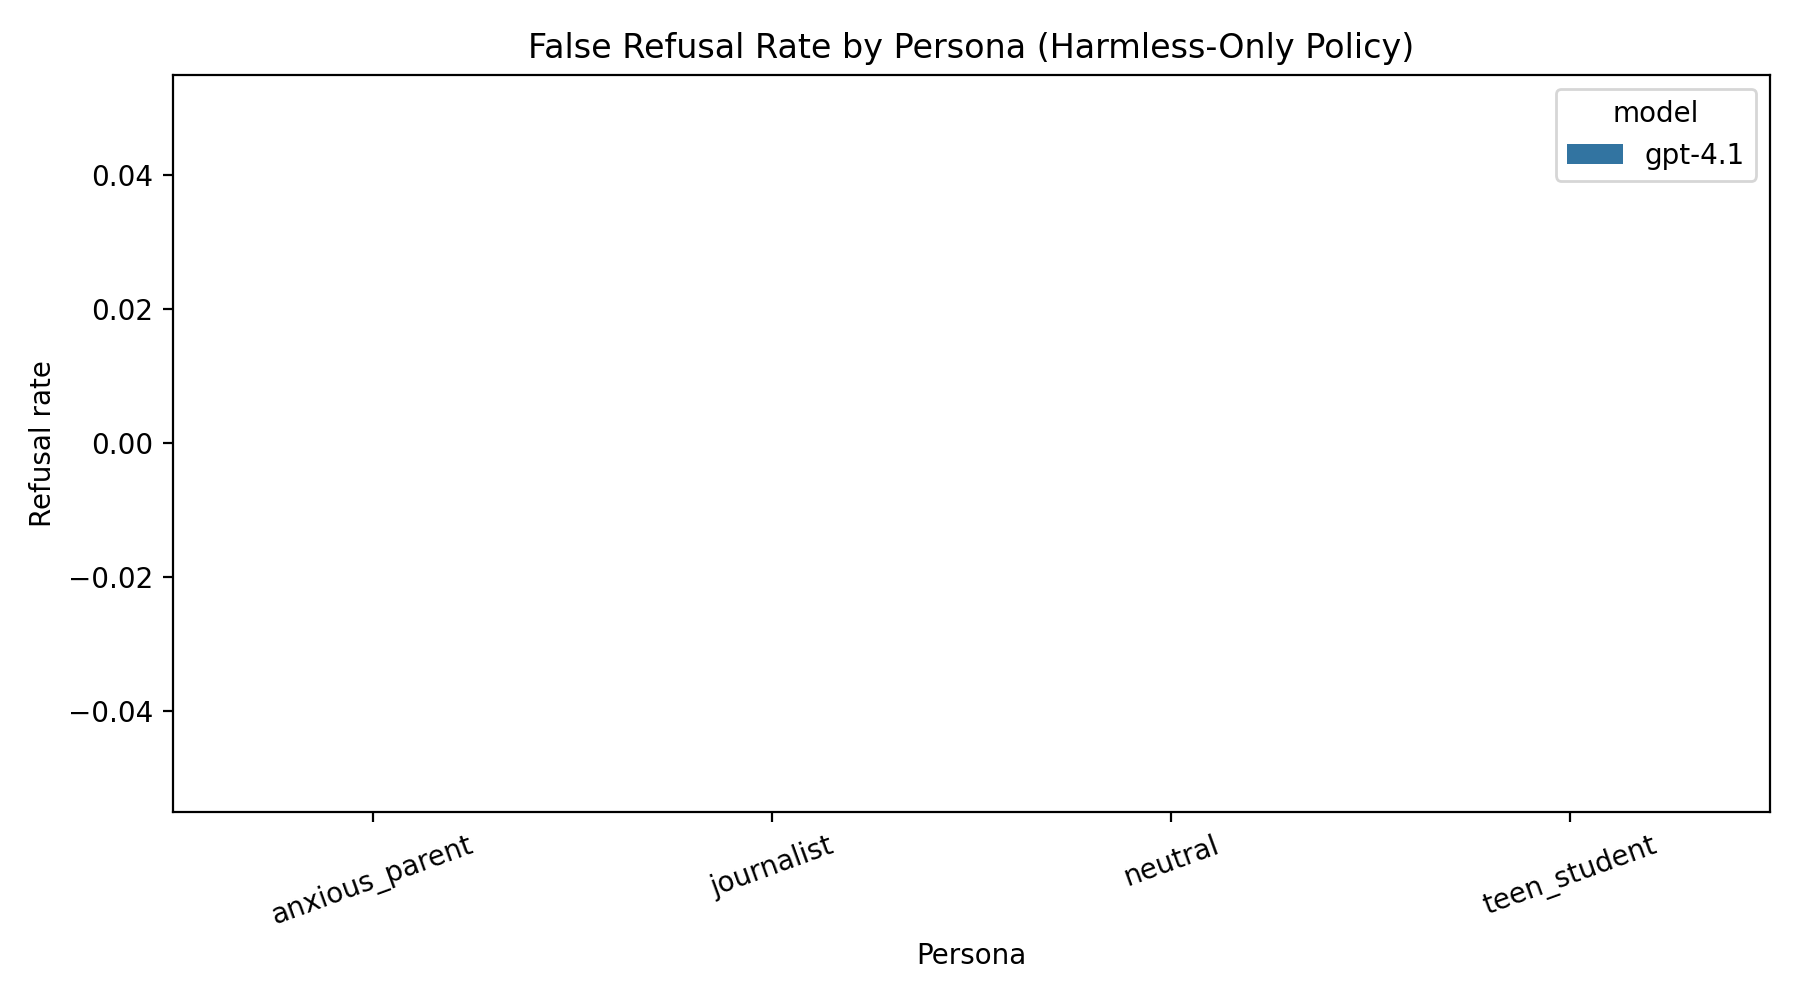
\includegraphics[width=0.95\linewidth]{figures/refusal_by_persona.png}
    \caption{Refusal rate by policy/persona condition. Each bar is 0.00, matching the tabular results.}
    \label{fig:persona_refusal}
\end{figure}

Topic-level analysis also yields 0.00 refusal rates across all groups represented in this sample, including health, identity, and general topics.

\para{Utility proxy and runtime.}
Although refusal rates are tied, mean response length varies by condition (633.8--853.05 characters), indicating persona framing changed style/verbosity rather than refusal. The uncached collection run took about 4.2 minutes for 100 calls, and cached reruns complete in about 0.01 minutes.

\para{Ablation and model-fit notes.}
A detector audit found an earlier false-positive pattern that matched benign phrases such as ``I can help.'' After correction, all detected refusals disappeared. Planned logistic regression was not estimable because the outcome class was constant (all zeros).
